\documentclass[10pt, letterpaper]{memoir}
\usepackage{HomeworkStyle}

\begin{document}
\begin{center}
	{\large Homework 11 -- Molecular Symmetry}
	
	Due: Monday, March 19 \hspace{3em} Points: ${\dfrac{~}{~~50~~}}$
\end{center}

Name: \rule[-.1mm]{15em}{0.1pt}	
	
	\section*{Problem 1 (10 points)}
	Give the correct point group for each molecule:
	
	\begin{itemize}
		\item Ethene (\ch{C2H4})
		
		\vspace{2em}
		\item 1,1-difluorethene (\ch{CF2CH2})
		
		\vspace{2em}
		\item Phosphorous pentachloride (\ch{PCl5})
		
		\vspace{2em}
		\item Ethane (\ch{C2H6}) in staggered conformation
		
		\vspace{2em}
		\item Phenol (\ch{C6H5OH}) in a completely planar conformation (OH lies in the plane)
		
		\vspace{2em}
	\end{itemize}

	\section*{Problem 2 (10 points)}
	The symmetry point groups have elements which fall into certain categories. Give a brief description of each type of symmetry element:
	
	\begin{description}
		\item[E]
		\vspace{1em}
		\item[C]
		
		\vspace{3em}
		\item[i]
		
		\vspace{3em}
		\item[$\sigma$]
		
		\vspace{3em}
		\item[S]
		
		\vspace{3em}
	\end{description}

	
	\newpage
	\section*{Problem 3 (20 points)}	
	Consider the trans-dichloroethene (\ch{CHClCHCl}) molecule. This molecule belongs to the $C_{2h}$ symmetry point group, whose character table is shown below:
	
	\begin{tabular}{c||c|c|c|c}
		$C_{2h}$ & $E$ & $C_2$ & $i$ & $\sigma_h$ \\ \midrule \midrule
		$A_g$ & $1$ & $1$ & $1$ & $1$ \\ \midrule
		$B_g$ & $1$ & $-1$ & $1$ & $-1$ \\ \midrule
		$A_u$ & $1$ & $1$ & $-1$ & $-1$ \\ \midrule
		$B_u$ & $1$ & $-1$ & $-1$ & $1$		
	\end{tabular}
	
	\noindent
	Give the correct irreducible symmetry representation for the following LCAOs and vibrations
	
	~
	
	\begin{tabular}{lr}
		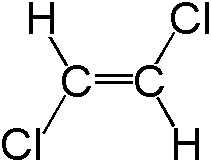
\includegraphics[width = 10em]{t_dichloroethene} \hspace{12em} & 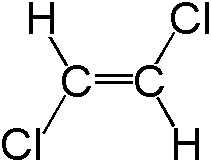
\includegraphics[width = 10em]{t_dichloroethene}\\ \\ \\ \\ \\
		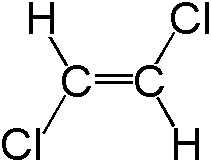
\includegraphics[width = 10em]{t_dichloroethene} \hspace{12em} & 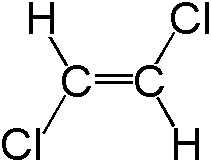
\includegraphics[width = 10em]{t_dichloroethene} \\ \\ \\ \\ \\
		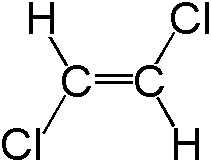
\includegraphics[width = 10em]{t_dichloroethene} \hspace{12em} & 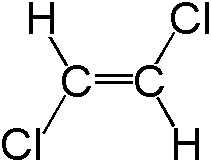
\includegraphics[width = 10em]{t_dichloroethene}\\ \\ \\ \\ 
	\end{tabular}
	
	\newpage
	\section*{Problem 4 (10 points)}
	Propadiene (common name Allene: \ch{CH2CCH2}) belongs to the $D_{2d}$ symmetry point group, whose character table is shown below:
	
	\begin{tabular}{c||c|c|c|c|c}
		$D_{2d}$ & $E$ & $2S_4$ & $C2$ & $2C^\prime 2$ & $2\sigma_d$ \\ \midrule \midrule
		$A_1$ & $1$ & $1$ & $1$ & $1$ & $1$ \\ \midrule
		$A_2$ & $1$ & $1$ & $1$ & $-1$ & $-1$\\ \midrule
		$B_1$ & $1$ & $-1$ & $1$ & $1$ & $-1$\\ \midrule
		$B_2$ & $1$ & $-1$ & $1$ & $-1$ & $1$\\ \midrule
		$E$ & $2$ & $0$ & $-2$ & $0$ & $0$
	\end{tabular}

	\noindent
	The set of non-vibrational nuclear motions has the characters: $\Gamma = $ $6$, $0$, $-2$, $-2$, $0$
	
	\noindent
	Decompose $\Gamma$ into its constituent irreducible representations
\end{document}
	